\chapter{Numeryczny rozmyty regulator SL}
	Rozmyty regulator typu SL jest w pewnym sensie podobny do rozmytego regulatora DMC, z dokładnością do tego, kiedy następuje rozmycie. Otóż w regulatorze SL rozmywana jest nie końcowa zmiana sterowania, a odpowiedzi skokowe regulatorów. W każdym kroku regulacji na podstawie poszczególnych odpowiedzi skokowych oraz aktualnych wag obliczana jest wspólna odpowiedź skokowa, a następnie następuje obliczane są nowe macierze $M$, $M^P$ i $M^{zP}$ na postawie których obliczana jest rozmyta odpowiedź swobodna obiektu, wykorzystywana do regulacji.
	
	Ponieważ wspomniany rozmyty algorytm SL miał zostać zaimplementowany w formie numerycznej zmienił się także sposób obliczania zmiany sterowania. Jest ona obliczana poprzez rozwiązanie problemu optymalizacji liniowo-kwadratowej przedstawionego wzorem \ref{eq:sl}, w którym $\tilde{y}^0$ oznacza rozmytą odpowiedź swobodną, a $M_k$ rozmytą macierz $M$. Problem ten w naszej implementacji rozwiązujemy za pomocą wbudowanej w Matlab funkcji minimalizacji $fmincon()$. W funkcji tej bierzemy także pod uwagę ograniczenia co do wielkości maksymalnej oraz minimalnej sterowania. Ograniczenia odnośnie maksymalnej zmiany sterowania w kroku po konsultacji z prowadzącym nie zostały wzięte pod uwagę.
	
	
	\begin{equation}
		min_{\Delta u}\{(y^{zad}-\tilde{y}^0-M_k*\Delta U)^T(y^{zad}-\tilde{y}^0-M_k*\Delta U)-\lambda \Delta u^T*\Delta u\}
		\label{eq:sl}
	\end{equation}
	
	\begin{figure}[h!]
		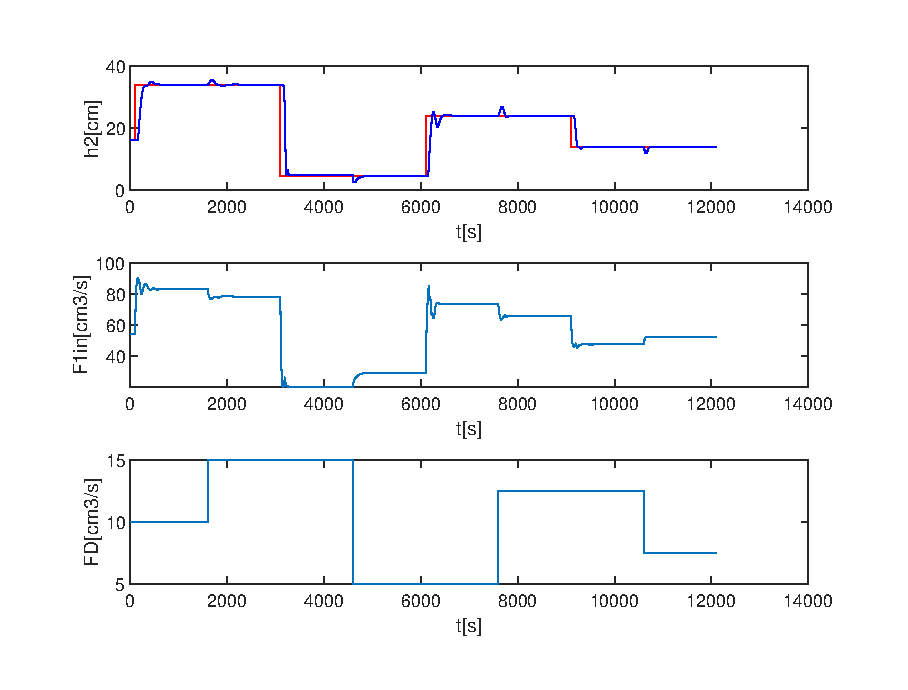
\includegraphics[width=0.9\linewidth]{plots/z3_fdmc_sl.eps}
		\caption{Przebieg regulacji dla numerycznego SL rozmytego}
		\label{rys:sl}
	\end{figure}
	
	
	Podczas sterowania regulatorem SL długości horyzontów, lambda oraz kształt funkcji przynależności przyjęte zostały takie same jak dla ostatniego przebiegu rozmytego regulatora DMC w zadaniu 2, czyli lambda równa 100, D równe 200, N równe 150, Nu równe 100, Dz równe 200 oraz funkcje przynależności tak jak na wykresie \ref{rys:dmcprzyn}.
	
	Przebieg regulacji umieszczony został an wykresie \ref{rys:sl}. Przebieg jest bardzo podobny do tego uzyskanego z rozmytego regulatora DMC, nie licząc okolic pierwszego skoku wartości zadanej wykresy praktycznie się nie różnią. Przy pierwszym skoku wartości zadanej algorytm SL działa jednakże nieco bardziej płynnie niż DMC. Przy regulacji DMC obiekt zwalnia przed dotarciem do wartości zadanej w formie pojedynczej oscylacji po czym dociera do niej praktycznie bez przeregulowania. Dla SL wykres jest płynniejszy, ale występuje wyraźne przekroczenie wartości zadanej. Błąd dla algorytmu SL wynosi jedynie 12.2571, więc jest zdecydowanie mniejszy niż błąd dla DMC. Oznacza to, że mimo wszystko wystąpiła poprawa regulacji.